%********************************************************************
% Kapitel 1
%*******************************************************
\chapter{Introduction}
\label{ch:Introduction}

\section{Motivation}

Given the continuous modernization of technologies nowadays, we believe that implementing a good recommendation engine will meet many of the interests of users who listen to music on a daily basis. In addition to Spotify, which is, along with iTunes, one of the largest music platforms in the world, our challenge has been to develop our own recommendation algorithm by adding some extras not present on these platforms.

Therefore, our task has not been to develop a complete music platform, but a tool that allows the user to discover new songs, playlists and artists according to their musical taste just using their Spotify account. In summary, the main aspects supporting the development of the application are the following:

\begin{itemize}
    \item It exists an increase demand on good recommender systems.
    \item Build a comprehensible and reliable recommender system for users, providing songs that they might like as well.
    \item Provide to users a different recommender system than the Spotify one, with new features, e.g., an option to rate the songs and display a rank for them.
    \item Focusing on the recommendation of songs, albums and artists, while Spotify is a more general application.
\end{itemize}

\section{Project Goals}

In general, all the requirements were met, thus mostly achieving all the objectives, which were to develop a web application capable of displaying songs, albums, and artists, using the Spotify API and our own recommender algorithm. Other pages such as the Dashboard Page or the Recently Played Page were also implemented.

On the other hand, this does not mean that a fully integrated application has been achieved, as some utilities can only be used through Spotify's own application. There have also been some API limitations in terms of fetching data. For instance, the maximum amount of songs that could be fetched from the Spotify API was 50. This meant that we had to use some other endpoints where we are able to fetch more songs and have a more reliable system.

With all of this, a more detailed explanation of the goals achieved and not achieved is given below.

\begin{itemize}
    \item Goals reached:
    \begin{itemize}
        \item Application developed according to the requirements:
        \begin{itemize}
            \item Dashboard page: This page displays two rows to the user, the first one shows the recently played songs and the second one shows the discover songs(recommended songs).
            \item Recently played page: This page shows the 50 most recent songs played by the user.
            \item Discover page: This page displays those songs that are recommended by our algorithm, based on the users record. It also has the possibility to filter by known tracks as well as by the user ratings. Furthermore, the user can also filter by music source and time range, depending on what time the songs were played for the last time.
        \end{itemize}
        \item Main objectives and requirements, e.g., discover functionality, were mostly achieved. It should be noted that in every page, the user can rate the songs as well as play them, being redirected to the Spotify main page.
    \end{itemize}
    \item Goals not reached:
    \begin{itemize}
        \item Filter by musical genre was not implemented, however, as we said before, we implemented time range settings as well as source settings, so the songs can be fetched from Top Tracks, Recently Played Songs, and also from an Example Playlist.
        \item Show the user the reason why we are recommending a song, album or artist or why not. We did not implement a function that allows the user to see why we recommended a song, album or artist.
        \item Possibility to play the song in our application instead of using the Spotify website. The user can not play the song in the application itself, but is redirected to the Spotify webpage.
        \item Usage of Deeplearning4j library and embeddings approach were not included to recommend songs.
    \end{itemize}
\end{itemize}

A comparison of the final application with the initial mock-up are shown below.

\begin{figure}[bth]
    \centering
    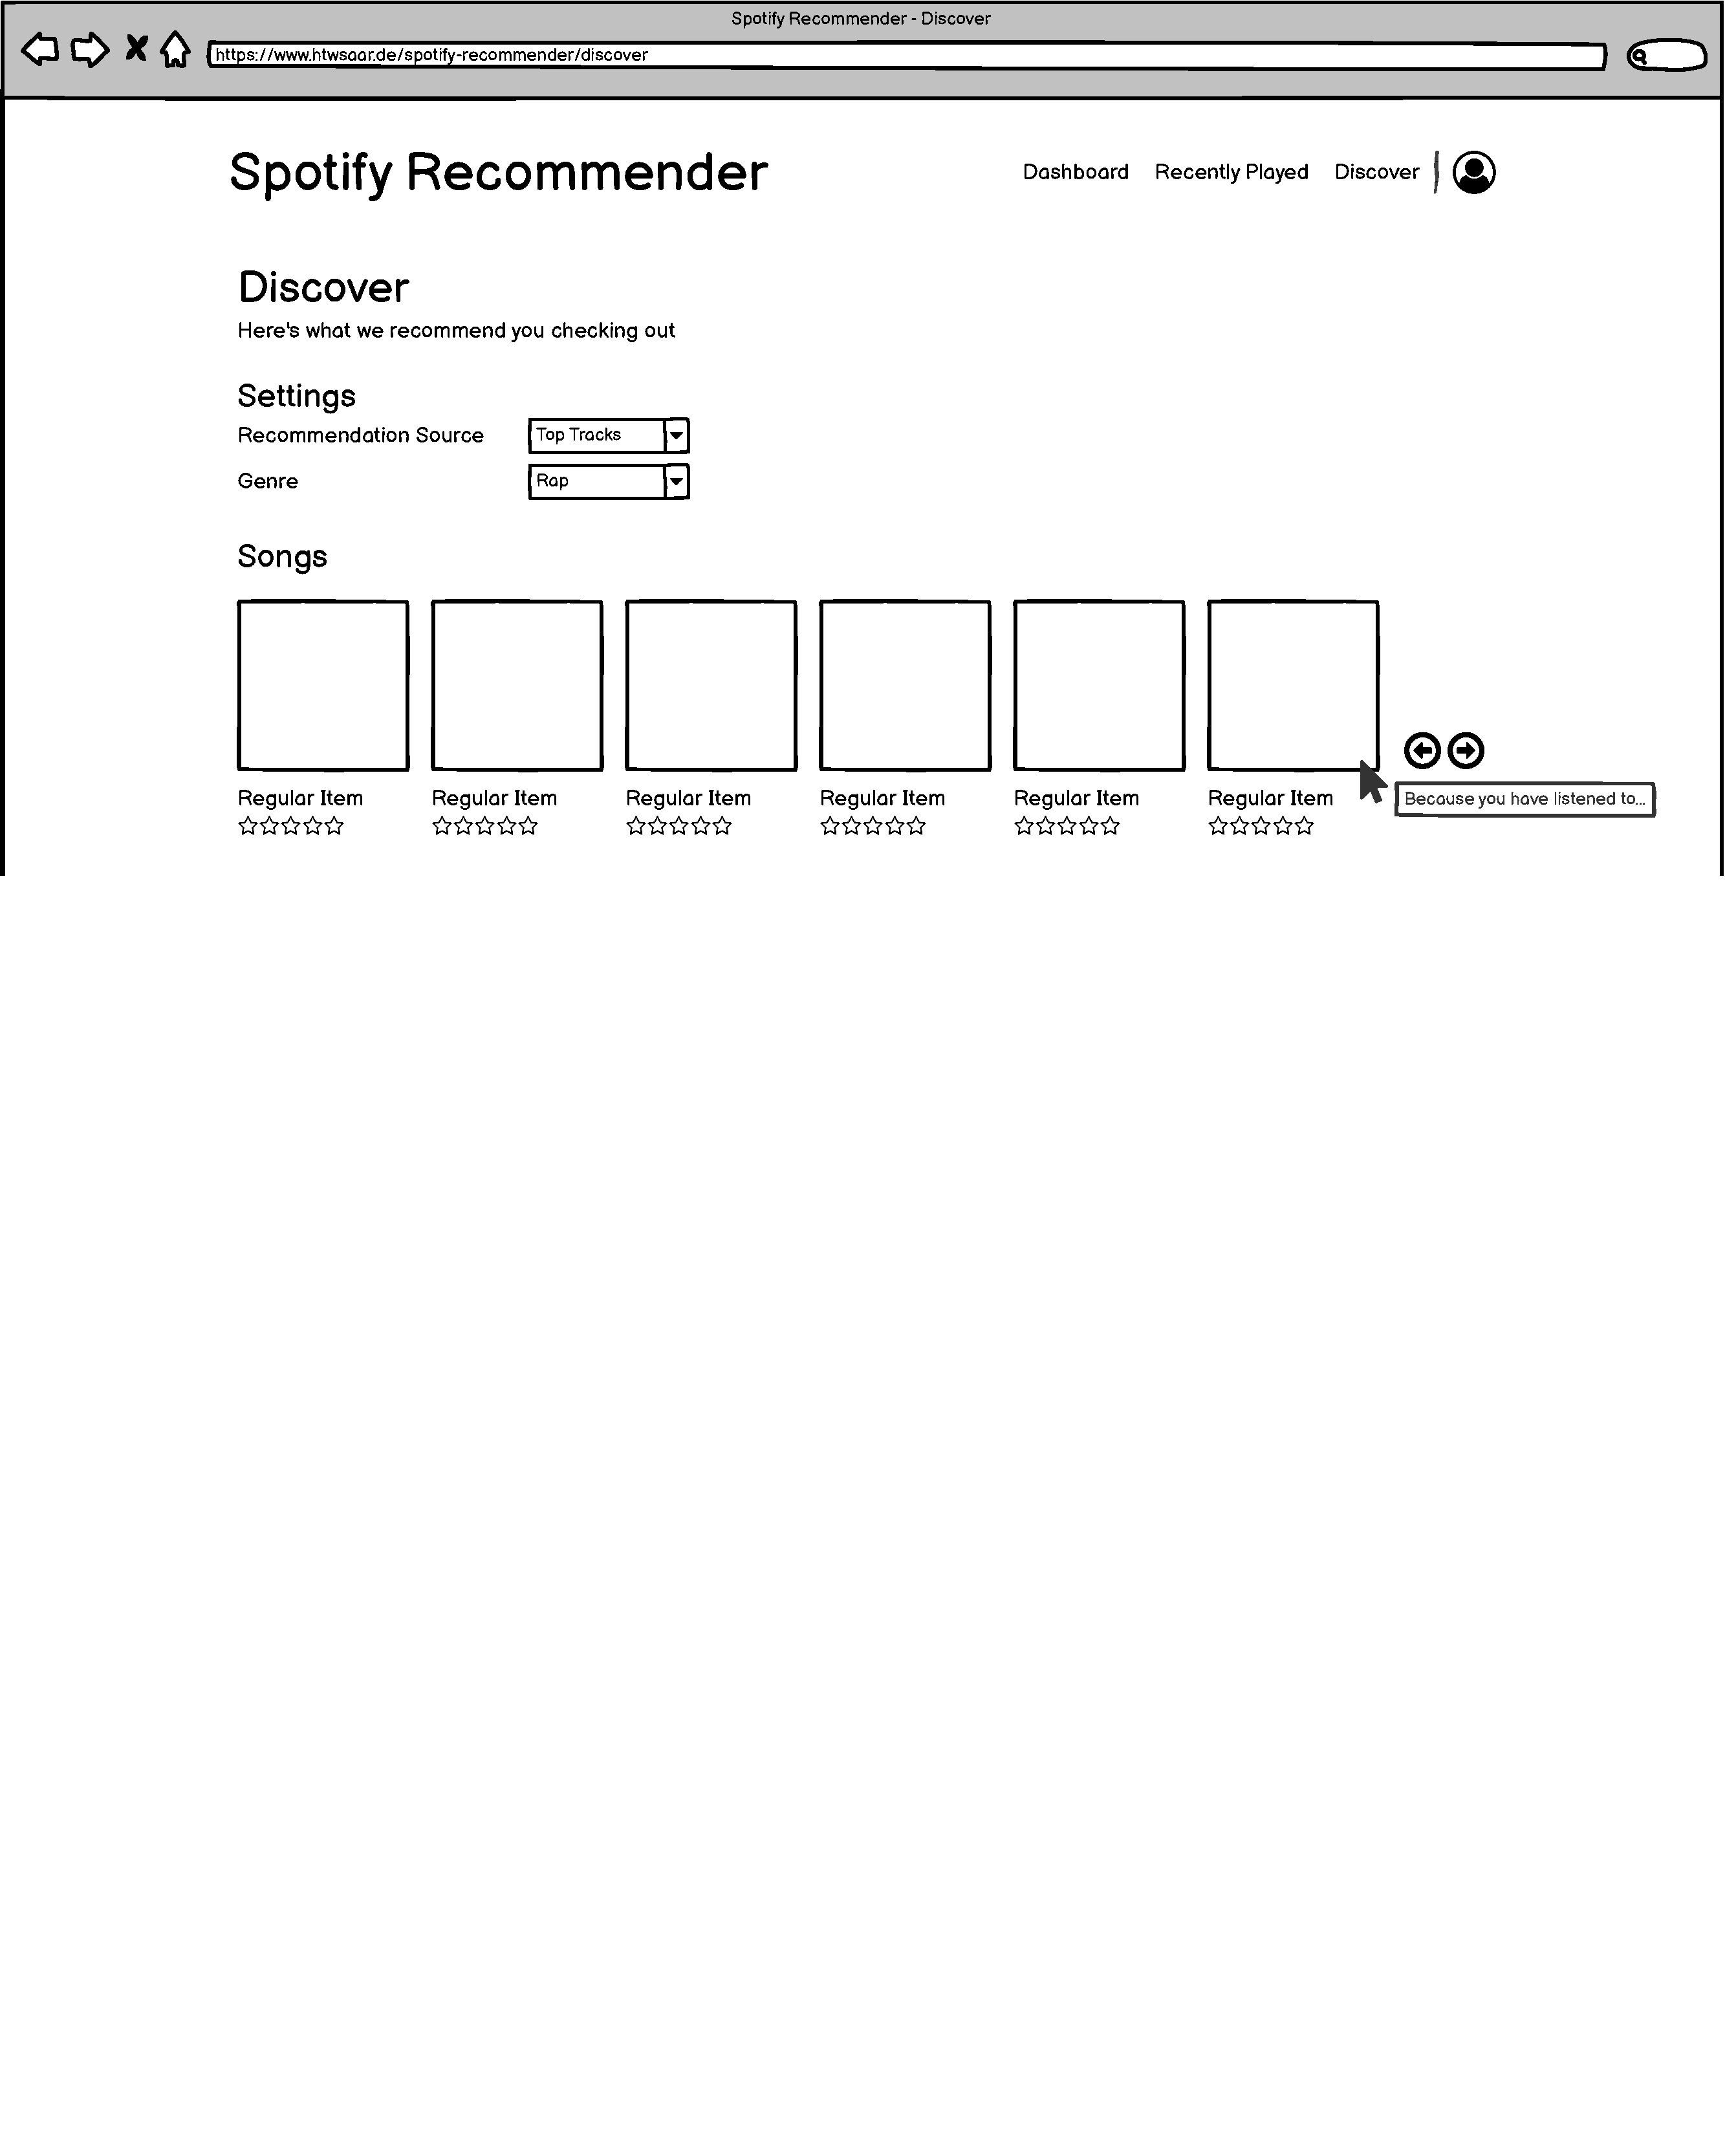
\includegraphics[width=1.0\textwidth]{Graphics/Chapter1/MockupDiscoverPage.pdf}
    \caption{Mockup Discover Page}
\end{figure}

\begin{figure}[bth]
    \centering
    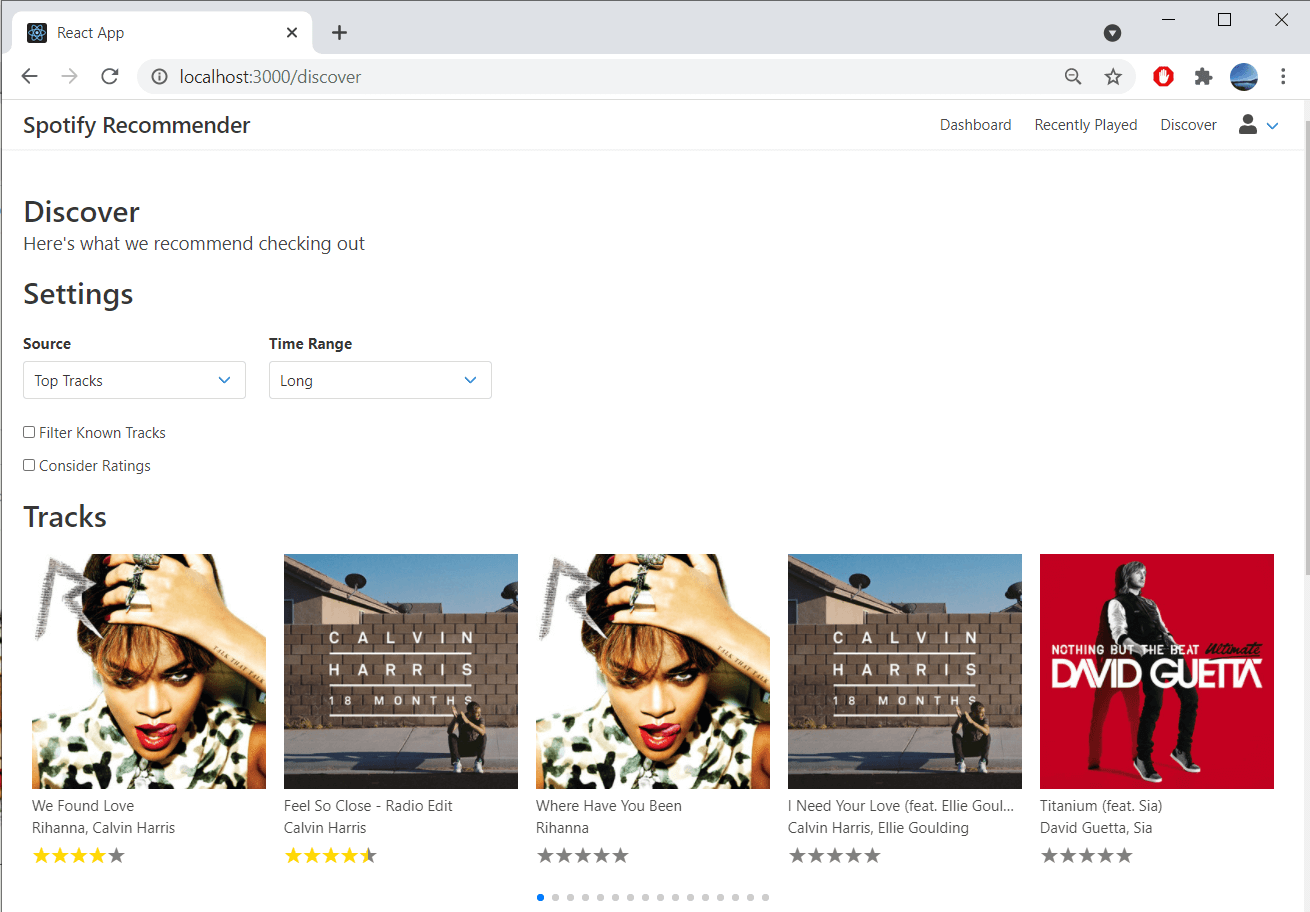
\includegraphics[width=1.0\textwidth]{Graphics/Chapter1/AppDiscoverPage.png}
    \caption{Final App Discover Page}
\end{figure}
